%!TEX program = xelatex
\documentclass[dvipsnames,svgnames,a4paper,11pt]{article}
% ----------------------------------------------------- 
%	加边框的命令
%	参考：https://tex.stackexchange.com/questions/531559/how-to-add-the-page-border-for-first-two-pages-in-latex
\usepackage{tikz}
\usetikzlibrary{calc}
\usepackage{eso-pic}
\AddToShipoutPictureBG{%
\begin{tikzpicture}[overlay,remember picture]
\draw[line width=0.6pt] % 边框粗细
    ($ (current page.north west) + (0.6cm,-0.6cm) $)
    rectangle
    ($ (current page.south east) + (-0.6cm,0.6cm) $); % 边框位置
\end{tikzpicture}}


\usepackage{xcolor}
\definecolor{c1}{HTML}{2752C9} % 目录颜色
\definecolor{c2}{RGB}{190,20,83} % 引用颜色

\usepackage{ctex}
\usepackage[top=28mm,bottom=28mm,left=15mm,right=15mm]{geometry} % 调整边距
\usepackage{hyperref} 
\hypersetup{
	colorlinks,
	linktoc = section, % 给目录加的超链接位置，选项有 section, page, all
	linkcolor = c1, % linkcolor 目录颜色
	citecolor = c1  % citecolor 引用颜色
}
\usepackage{amsmath,enumerate,multirow,float}
\usepackage{tabularx}
\usepackage{tabu}
\usepackage{subfig}
\usepackage{fancyhdr}
\usepackage{graphicx}
\usepackage{wrapfig}  
\usepackage{physics}
\usepackage{appendix}
\usepackage{amsfonts,amssymb}
% \usepackage{annotate-equations} % 公式标注（未安装，已禁用）
\usepackage{pgfplots} % pgf 绘图


% ---------------------------------------------------------------------
%	定义了两类colorbox
\usepackage{tcolorbox}
\tcbuselibrary{skins,breakable}
\newtcolorbox{tbox}[2][]{
    colframe=black!70!,
    breakable,
    enhanced, % 跨页后不会显示下边框
    boxrule =0.5pt,
    title = {#2},
    fonttitle = \large\bfseries,
    drop fuzzy shadow,
    #1
}
\newtcolorbox[auto counter,number within=section]{question}[1][]{
  top=2pt,bottom=2pt,arc=1mm,
  boxrule=0.5pt,
  breakable,
  enhanced, % 跨页后不会显示下边框
  coltitle=c1!80!gray,
  colframe=c1,
  colback=c1!3!white,
  drop fuzzy shadow,
  title={思考题~\thetcbcounter：\quad},
  fonttitle=\bfseries,
  attach title to upper,
  #1
}

% ---------------------------------------------------------------------
%	利用 cleveref 改变引用格式，\cref 是引用命令
\usepackage{cleveref}
\crefformat{figure}{#2{\textcolor{c2}{图 #1}}#3} % 图片的引用格式
\crefformat{equation}{#2{(\textcolor{c2}{#1})}#3} % 公式的引用格式
\crefformat{table}{#2{\textcolor{c2}{表 #1}}#3} % 表格的引用格式

% ---------------------------------------------------------------------
%	页眉页脚设置
\fancypagestyle{plain}{\pagestyle{fancy}}
\pagestyle{fancy}
\lhead{\kaishu 中山大学物理与天文学院物理实验\uppercase\expandafter{\romannumeral3}} % 左边页眉，学院 + 课程
\rhead{\kaishu Template 实验报告模板} % 右边页眉，实验报告标题
\cfoot{\thepage} % 页脚，中间添加页码
\setlength{\headheight}{13.6pt}

% ---------------------------------------------------------------------
%	对目录、章节标题的设置
\renewcommand{\contentsname}{\centerline{\huge 目录}}
% titlesec/titletoc 与 ctex 冲突，已禁用
% \usepackage{titlesec}
% \usepackage{titletoc}
% \titleformat{\section}{\centering\LARGE}{}{1em}{}
% \newcommand{\nsection}[3]{%
%     \section{#1 #2 \hspace{11pt} \textbf{#3}}%
% }

% ---------------------------------------------------------------------
%   listing代码环境设置
\usepackage{listings}
\lstloadlanguages{python}
\lstdefinestyle{pythonstyle}{
backgroundcolor=\color{gray!5},
language=python,
frameround=tftt,
frame=shadowbox, 
keepspaces=true,
breaklines,
columns=spaceflexible,                   
basicstyle=\ttfamily\small, % 基本文本设置，字体为 teletype，大小为 small
keywordstyle=[1]\color{c1}\bfseries, 
keywordstyle=[2]\color{Red!70!black},   
stringstyle=\color{Purple},       
showstringspaces=false,
commentstyle=\ttfamily\scriptsize\color{green!40!black}, % 注释文本设置，字体为 teletype，大小为 scriptsize
tabsize=2,
morekeywords={as},
morekeywords=[2]{np, plt, sp},
numbers=left, % 代码行数，位置在左
numberstyle=\it\tiny\color{gray}, % 代码行数的数字字体设置
stepnumber=1,
rulesepcolor=\color{gray!30!white}
}


% ---------------------------------------------------------------------
%	将表格封装起来
\newcommand{\scoresTable}[8]{
    \begin{table}
        \renewcommand\arraystretch{1.7}
        \begin{tabularx}{\textwidth}{
                |X|X|X|X
                |X|X|X|X|}
            \hline
            \multicolumn{2}{|c|}{预习报告} & \multicolumn{2}{|c|}{实验记录} & \multicolumn{2}{|c|}{分析讨论} & \multicolumn{2}{|c|}{总成绩} \\
            \hline
            \centering#1&\centering#2 &\centering#3 &\centering#4 &\centering#5 &\centering#6 &\centering#7 &{\centering#8} \\
            \hline
        \end{tabularx}
    \end{table}
}
\newcommand{\infoTable}[6]{
    \begin{table}
        \renewcommand\arraystretch{1.7}
        \begin{tabularx}{\textwidth}{|X|X|X|X|}
        \hline
        专业：& #1 &年级：& #2\\
        \hline
        姓名：& #3   & 学号：&#4\\
        \hline
        实验时间：&#5 & 教师签名：&#6 \\
        \hline
        \end{tabularx}
    \end{table}
}

% ---------------------------------------------------------------------
%	其他设置
\def\degree{${}^{\circ}$} % 角度
\graphicspath{{./}{./images/}} % 插入图片的相对路径
\allowdisplaybreaks[4]  %允许公式跨页

\usetikzlibrary{patterns,decorations.markings,arrows.meta,bending} % TikZ 包的拓展

\pgfplotsset{compat=1.18}
\graphicspath{{./}{images/}{figures/}}
\usepackage{booktabs}
\usepackage{caption}
\hypersetup{pdftitle={从零训练 MNIST DDPM 实验报告},pdfauthor={请填写姓名}}
\lhead{\kaishu MNIST DDPM 实验报告}
\rhead{\kaishu 课程后编程实验}

\begin{document}
\ClearShipoutPictureBG
\begin{titlepage}
\thispagestyle{empty}
\begin{center}
\vspace*{0.25cm}

\includegraphics[width=0.40\textwidth]{images/school_flat.png}\par
\vspace{0.55cm}
{\fontsize{28pt}{34pt}\selectfont\bfseries 课程后编程实验报告\par}
\vspace{0.65cm}
{\fontsize{24pt}{30pt}\selectfont\bfseries 从零训练 MNIST 扩散模型\par}
\vspace{1.4cm}
{\fontsize{17pt}{23pt}\selectfont
\begin{tabular}{p{0.22\textwidth}p{0.48\textwidth}}
学院： & \underline{\makebox[0.36\textwidth][c]{电子信息与通信学院}} \\
专业班级： & \underline{\makebox[0.36\textwidth][c]{电信2303班}} \\
姓名： & \underline{\makebox[0.36\textwidth][c]{赵浩宇}} \\
学号： & \underline{\makebox[0.36\textwidth][c]{U202314553}} \\
指导教师： & \underline{\makebox[0.36\textwidth][c]{王兴刚}} \\
\end{tabular}}
\end{center}
\end{titlepage}

\begingroup\small\setlength{\parskip}{0pt}\tableofcontents\endgroup
\clearpage

\section{实验目的与数据}
本实验从零实现一个用于 MNIST 手写数字生成的去噪扩散概率模型（DDPM）。实验重点不是追求分类意义上的“跑分”，而是验证扩散模型的前向加噪、噪声预测网络和反向生成链路，并分析反向采样步数对质量与速度的影响。

使用 torchvision 下载的 MNIST 训练集包含 60,000 张 $28\times28$ 灰度图像，像素经标准化后落在 $[-1,1]$。本次训练共进行 20 个 epoch，批大小为 128，学习率为 $2\times10^{-4}$，扩散步数为 1000，随机种子为 42。训练环境为 AutoDL 单张 NVIDIA GeForce RTX 3080 Ti；最终 checkpoint 记录了 9,380 个优化 step。

\section{方法与软件实现}
\subsection{前向加噪}
设 $x_0$ 为真实图像，线性噪声日程定义为 $\beta_t\in[10^{-4},0.02]$，$\alpha_t=1-\beta_t$，$\bar\alpha_t=\prod_{s=1}^{t}\alpha_s$。利用闭式表达式直接采样：
\begin{equation}
 q(x_t|x_0)=\mathcal N\left(\sqrt{\bar\alpha_t}x_0,(1-\bar\alpha_t)I\right),\qquad
 x_t=\sqrt{\bar\alpha_t}x_0+\sqrt{1-\bar\alpha_t}\,\epsilon,
\end{equation}
其中 $\epsilon\sim\mathcal N(0,I)$。这避免了逐步执行前向马尔可夫链。

\subsection{去噪网络与损失}
去噪器是时间条件 Tiny U-Net，使用正弦时间嵌入、残差块、GroupNorm、SiLU 激活和跳跃连接。实际可训练参数量为 670,561，满足不超过 5M 的要求。训练目标为预测加入图像的噪声：
\begin{equation}
 \mathcal L=\mathbb E_{x_0,t,\epsilon}\left[\|\epsilon-\epsilon_\theta(x_t,t)\|_2^2\right].
\end{equation}

\subsection{反向 ancestral sampling}
推理时从 $x_T\sim\mathcal N(0,I)$ 开始，依据网络预测噪声逐步计算 $x_{t-1}$，除最后一步外加入后验方差对应的随机噪声。程序实现了完整 1000 步采样，并实现了从同一条 1000 步噪声日程均匀抽取 200 或 50 个时间点的跳步 ancestral sampling。

\section{实验结果与分析}
\subsection{训练损失}
\begin{figure}[H]
\centering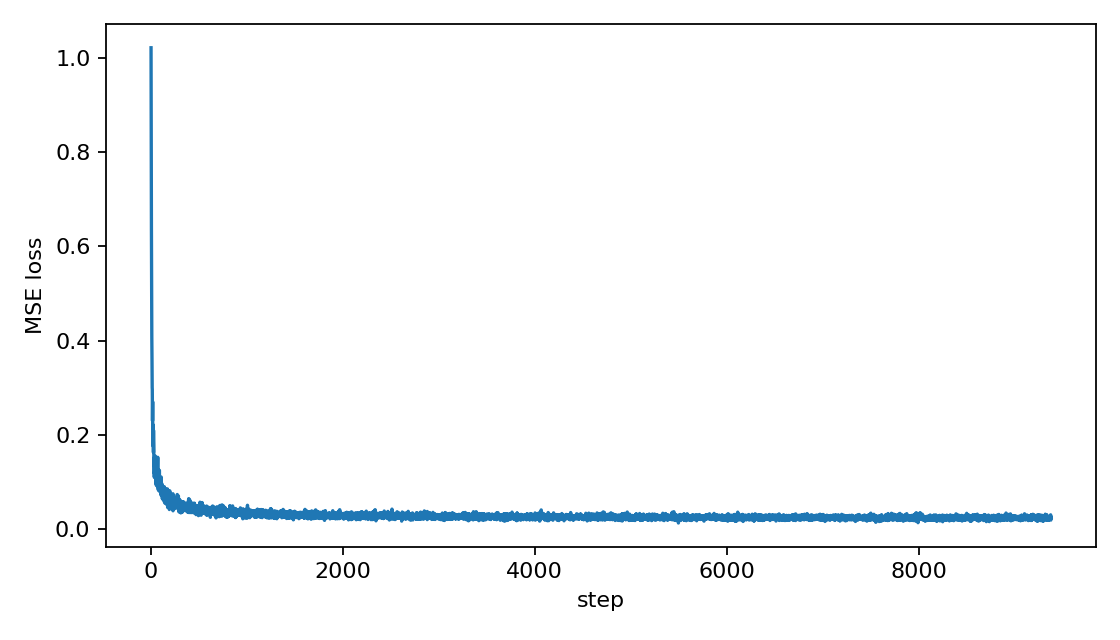
\includegraphics[width=0.82\textwidth]{figures/loss.png}
\caption{20 个 epoch 的 MSE 噪声预测损失曲线。}
\label{fig:loss}
\end{figure}
如图~\ref{fig:loss} 所示，损失在训练初期快速下降，随后在约 0.02--0.04 附近波动并趋于稳定，说明网络已经学会了基本的噪声估计。后期仍存在小幅随机波动，这是随机抽取时间步和训练 batch 带来的正常现象。

\subsection{生成样本}
\begin{figure}[H]
\centering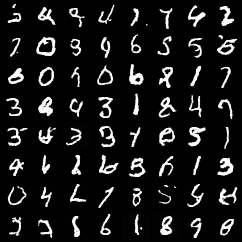
\includegraphics[width=0.38\textwidth]{figures/samples_final.png}
\caption{完整 1000 步反向采样得到的 8$\times$8 样本网格。}
\label{fig:sample}
\end{figure}
样本整体能够呈现 MNIST 数字的笔画结构，说明模型已经完成从高斯噪声到数字图像分布的迁移。但部分数字仍有变形、粘连和类别边界不清晰的问题，表明在较小网络和有限训练轮数下，生成质量仍有提升空间。

\subsection{采样步数对比}
为便于复现实验，本地 CPU 上对同一 checkpoint、同一批 64 个样本进行测量，结果如表~\ref{tab:time}。实际训练和服务器推理使用 AutoDL 单张 RTX 3080 Ti；耗时会受到硬件、CUDA 版本和线程设置影响，因此表中重点关注相对趋势。
\begin{table}[H]
\centering
\caption{不同反向采样步数的耗时对比（CPU，64 张图）。}
\label{tab:time}
\begin{tabular}{rrrr}
\toprule
采样步数 & 总耗时/s & 每张图/s & 相对 1000 步耗时 \\
\midrule
1000 & 58.1132 & 0.9080 & 100\% \\
200  & 12.2095 & 0.1908 & 21.0\% \\
50   & 2.9715  & 0.0464 & 5.1\% \\
\bottomrule
\end{tabular}
\end{table}

\begin{figure}[H]
\centering
\subfloat[1000 步]{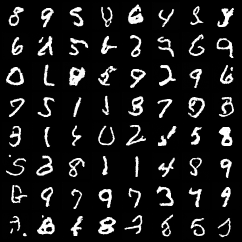
\includegraphics[width=0.30\textwidth]{figures/steps_1000.png}}
\quad\subfloat[200 步]{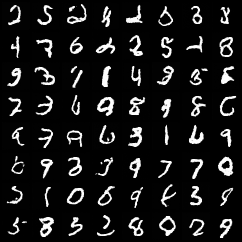
\includegraphics[width=0.30\textwidth]{figures/steps_200.png}}
\quad\subfloat[50 步]{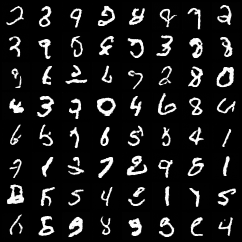
\includegraphics[width=0.30\textwidth]{figures/steps_50.png}}
\caption{不同采样步数下的生成样本。}
\label{fig:steps}
\end{figure}

从图~\ref{fig:steps} 可以看到，1000 步样本的笔画相对完整，200 步仍能保持大部分数字结构，而 50 步虽然速度最快，但更容易出现断笔、模糊和形状异常。该结果体现了扩散采样中质量与推理成本之间的典型折中：从 1000 步降到 50 步，速度约提升 19.6 倍，但质量有明显损失。服务器 GPU 上的绝对时间会更短，不过三种设置的相对比较仍具有参考价值。

\section{问题、解决方法与总结}
实验中首先遇到时间条件残差块调用参数遗漏的问题，导致模型前向传播报错；补齐各层的时间嵌入后解决。随后发现部分 PyTorch 版本不支持顶层 `torch.silu` 接口，改用 `torch.nn.functional.silu` 提高了兼容性。另一个需要注意的问题是，200/50 步对比不能简单重新构造一条 50 步噪声日程，否则模型训练时的时间语义会改变；本实验采用训练好的 1000 步日程均匀跳步，比较更公平。

本实验验证了 DDPM 从数据预处理、前向扰动、噪声预测到反向生成的完整流程。结果表明，小型 U-Net 已能生成可辨认的 MNIST 数字；采样步数是影响推理速度的直接因素，实际应用中可根据质量要求选择 200 步或进一步采用 DDIM 等确定性加速方法。

\end{document}
